\chapter{Giải thuật di truyền đề xuất giải bài toán tối ưu thời gian sống của mạng cảm biến không dây ngầm}
Với việc sử dụng giải thuật di truyền để tối ưu hóa hàm mục tiêu, ta chọn một cá thể là tập các vị trí được chọn để triển khai relay, việc thiết lập kết nối giữa relays và sensors sẽ được thực hiện với từng cá thể, cuối cùng sử dụng hàm thích nghi để đánh giá cá thể này.
\section{Mã hóa cá thể}
Dựa theo biến quyết định $z$ trong mô hình bài toán, một cách tự nhiên ta chọn mã hóa nhị phân để biểu diễn lời giải.
\\Nhắc lại: $z = (z_1, z_2,…, z_m)$ trong đó $z_j$ = 1 nếu vị trí $j$ được chọn để triển khai relay

Ví dụ: một cá thể với 10 vị trí khả thi đặt relay

\begin{figure}[h]
    \centering
    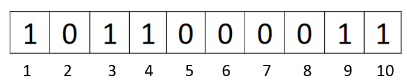
\includegraphics[width=10cm]{picture/indi_encoding.png}
    \caption{Mã hóa cá thể }
\end{figure}

\section{Xác định các vị trí đặt relay}
\subsection{Khởi tạo quần thể}
Khởi tạo ngẫu nhiên: đây là cách khởi tạo rất đơn giản, tạo ngẫu nhiên một số dãy nhị phân độ dài $m$ trong đó không có dãy nào chỉ chứa phần tử 0.
\subsection{Lai ghép}
Đề xuất sử dụng phép lai ghép một điểm cắt cho hai cá thể $z_1$, $z_2$ được chọn ngẫu nhiên từ quần thể hiện tại. Trong phép lai ghép một điểm cắt, ta chọn tùy ý một điểm làm điểm cắt, sau đó ghép các đoạn gen của cha mẹ lại để tạo ra hai cá thể con 
\\Minh họa cho phép lai ghép như sau
\begin{figure}[H]
    \centering
    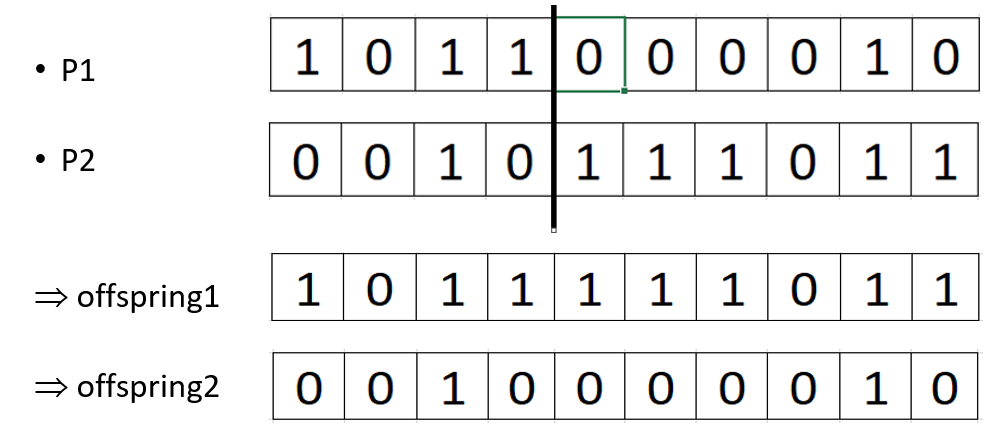
\includegraphics[width=0.8\linewidth]{picture/crossover.png}
    \caption{Toán tử lai ghép}
\end{figure}
%picture
\subsection{Đột biến }
Cá thể con sau khi sinh ra có thể xảy ra đột biến với xác suất đột biến $q$. Phép đột biến được thực hiện như sau: chọn ngẫu nhiên hai gen trên cá thể trong đó một gen mang giá trị 1 và một gen mang giá trị 0, sau đó đổi chỗ chúng cho nhau.
\begin{figure}[H]
    \centering
    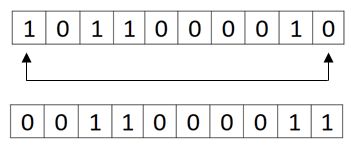
\includegraphics[width=0.6\linewidth]{picture/mutation.png}
    \caption{Toán tử đột biến}
\end{figure}
\section{Xác định kết nối giữa relays và sensors }
Dựa vào các toán tử lai ghép và đột biến của giải thuật di truyền, quần thể có được độ đa dạng tương đối và khả năng lớn sẽ hội tụ về hướng lời giả tối ưu, do đó sau khi cố định các vị trí đặt relay, ta sử dụng một thuật toán heuristic đơn giản để tạo các kết nối giữa các sensors – relays nhằm làm tăng tốc độ giải thuật.

\begin{algorithm}[ht]
    \SetKwData{Selid}{$sel\_id$}
    \SetKwData{Minmax}{min\_max}
    \SetKwData{Localmax}{local\_max}
    \SetKwData{lossone}{$loss_1$}
    \SetKwData{losstwo}{$loss_2$}
    \SetKwData{Sensors}{S}
    \SetKwData{Relays}{R}
    \SetKwData{Connect}{C}
    \SetKwData{TRUE}{True}
    \SetKwData{FALSE}{False}
    \SetKwData{esensor}{$Et$}
    \SetKwData{erelay}{$Er$}
    \SetKwData{varlthree}{$l_3$}
    \SetKwFunction{MAX}{Max}
    \SetKwFunction{ASSIGN}{Assign}
    \SetKwInOut{Input}{Đầu vào}
    \SetKwInOut{Output}{Đầu ra}
    \Input{
        \\ \Sensors = $\{s_1, s_2, ..., s_n\}$ : tập các sensors 
        \\ \Relays = $\{r_1, r_2, ..., r_n\}$: tập các relays 
        \\ \Connect: ma trận kết nối 
        \\ \esensor, \erelay: năng  lượng tiêu hao của sensors và relays}
    \Output{\\Các kết nối giữa sensors và relays}
        \SetAlgoLined
        \BlankLine
        \Begin{
            \For{$s_n \in \{s_1, s_2, ..., s_n\}$}{
                $\Minmax \leftarrow$ INF \\
                $\Selid \leftarrow 0$ \\
                \For{$r_n \in \{r_1, r_2, ..., r_n\}$}{
                    $\lossone \leftarrow \esensor_{i, \Selid}$   \\
                    $\losstwo \leftarrow \erelay_j$ \\
                    $\Localmax \leftarrow \MAX(\lossone, \losstwo)$ \\
                    \If {\Minmax < \Localmax} {
                        $\Minmax \leftarrow \Localmax$ \\
                        $\Selid  \leftarrow j$
                    }
                }
                $\ASSIGN ~s_i$ to $r_{\Selid}$
            }
            % $\START \leftarrow \ivar$\\
            % $\END \leftarrow \jvar$\\
            % $\MID \leftarrow \floor{(\START + \END)/2}$\\
            % $\varlone \leftarrow \MaxFlow (e'_1, ..., e'_{start})$\\
            % $\varltwo \leftarrow \MaxFlow (e'_1, ..., e'_{mid})$\\
            % $\varlthree \leftarrow \MaxFlow (e'_1, ..., e'_{end})$\\
            % \If{\varlone is \TRUE} {
            % return $\{e'_1, ..., e'_{start}\}$
            % }\If{\varlthree is \FALSE} {
            % return \FALSE
            % }
            % \eIf{\varltwo is \FALSE} {
            %     return \FindConnect ($E', mid, end$)
            % }{
            %     return \FindConnect ($E', start, mid$)
            % }
            % \DecMargin{1em}
        }
        \caption{Connect ($S, R, C, Et, Er$)}      
    \end{algorithm}
\section{Hàm thích nghi và chọn lọc cá thể}
Trong đề xuất này, ta sử dụng hàm mục tiêu của bài toán như là hàm thích nghi chính của mỗi cá thể. Với hai cá thể có giá trị hàm thích nghi chính tương đương, thuật toán sử dụng thêm hàm mục tiêu phụ là tổng năng lượng tiêu hao của các nút trong mạng.

Sau khi tiến hành lai ghép, đột biến, các cá thể sẽ được tính độ thích nghi và sắp xếp theo giá trị thích nghi này. Các cá thể tốt nhất sẽ được giữ lại để tiếp tục quá trình tiến hóa còn các cá thể tồi hơn sẽ bị loại bỏ. Đây là phương pháp chọn lọc giữ lại những cá thể ưu tú.

Phần trên trình bày giải thuật di truyền đề xuất  giải quyết bài toán tối ưu tuổi thọ mạng cảm biến không dây ngầm, giải thuật này được đặt tên là GAH.